\section{实验结果}

\subsection{板级验证结果}

将生成的比特流文件下载到Nexys DDR开发板后，进行以下验证：

\begin{enumerate}[leftmargin=2em]
    \item 将 \texttt{choose} 开关拨至 \texttt{00}（显示数据存储器结果）。
    \item 按下复位按钮后释放，CPU开始执行测试程序。
    \item 观察数码管显示。
\end{enumerate}

\textbf{预期结果}：

\begin{itemize}[leftmargin=2em]
    \item 数码管低半字（低4位数码管）显示 \texttt{0001}，表示全部11个测试函数通过。
    \item 数码管高半字（高4位数码管）持续递增，表示时钟中断功能正常。
\end{itemize}

\textbf{实际验证}：


\begin{figure}[H]
    \centering
    % TODO: 替换为数码管显示0001的开发板实物照片
    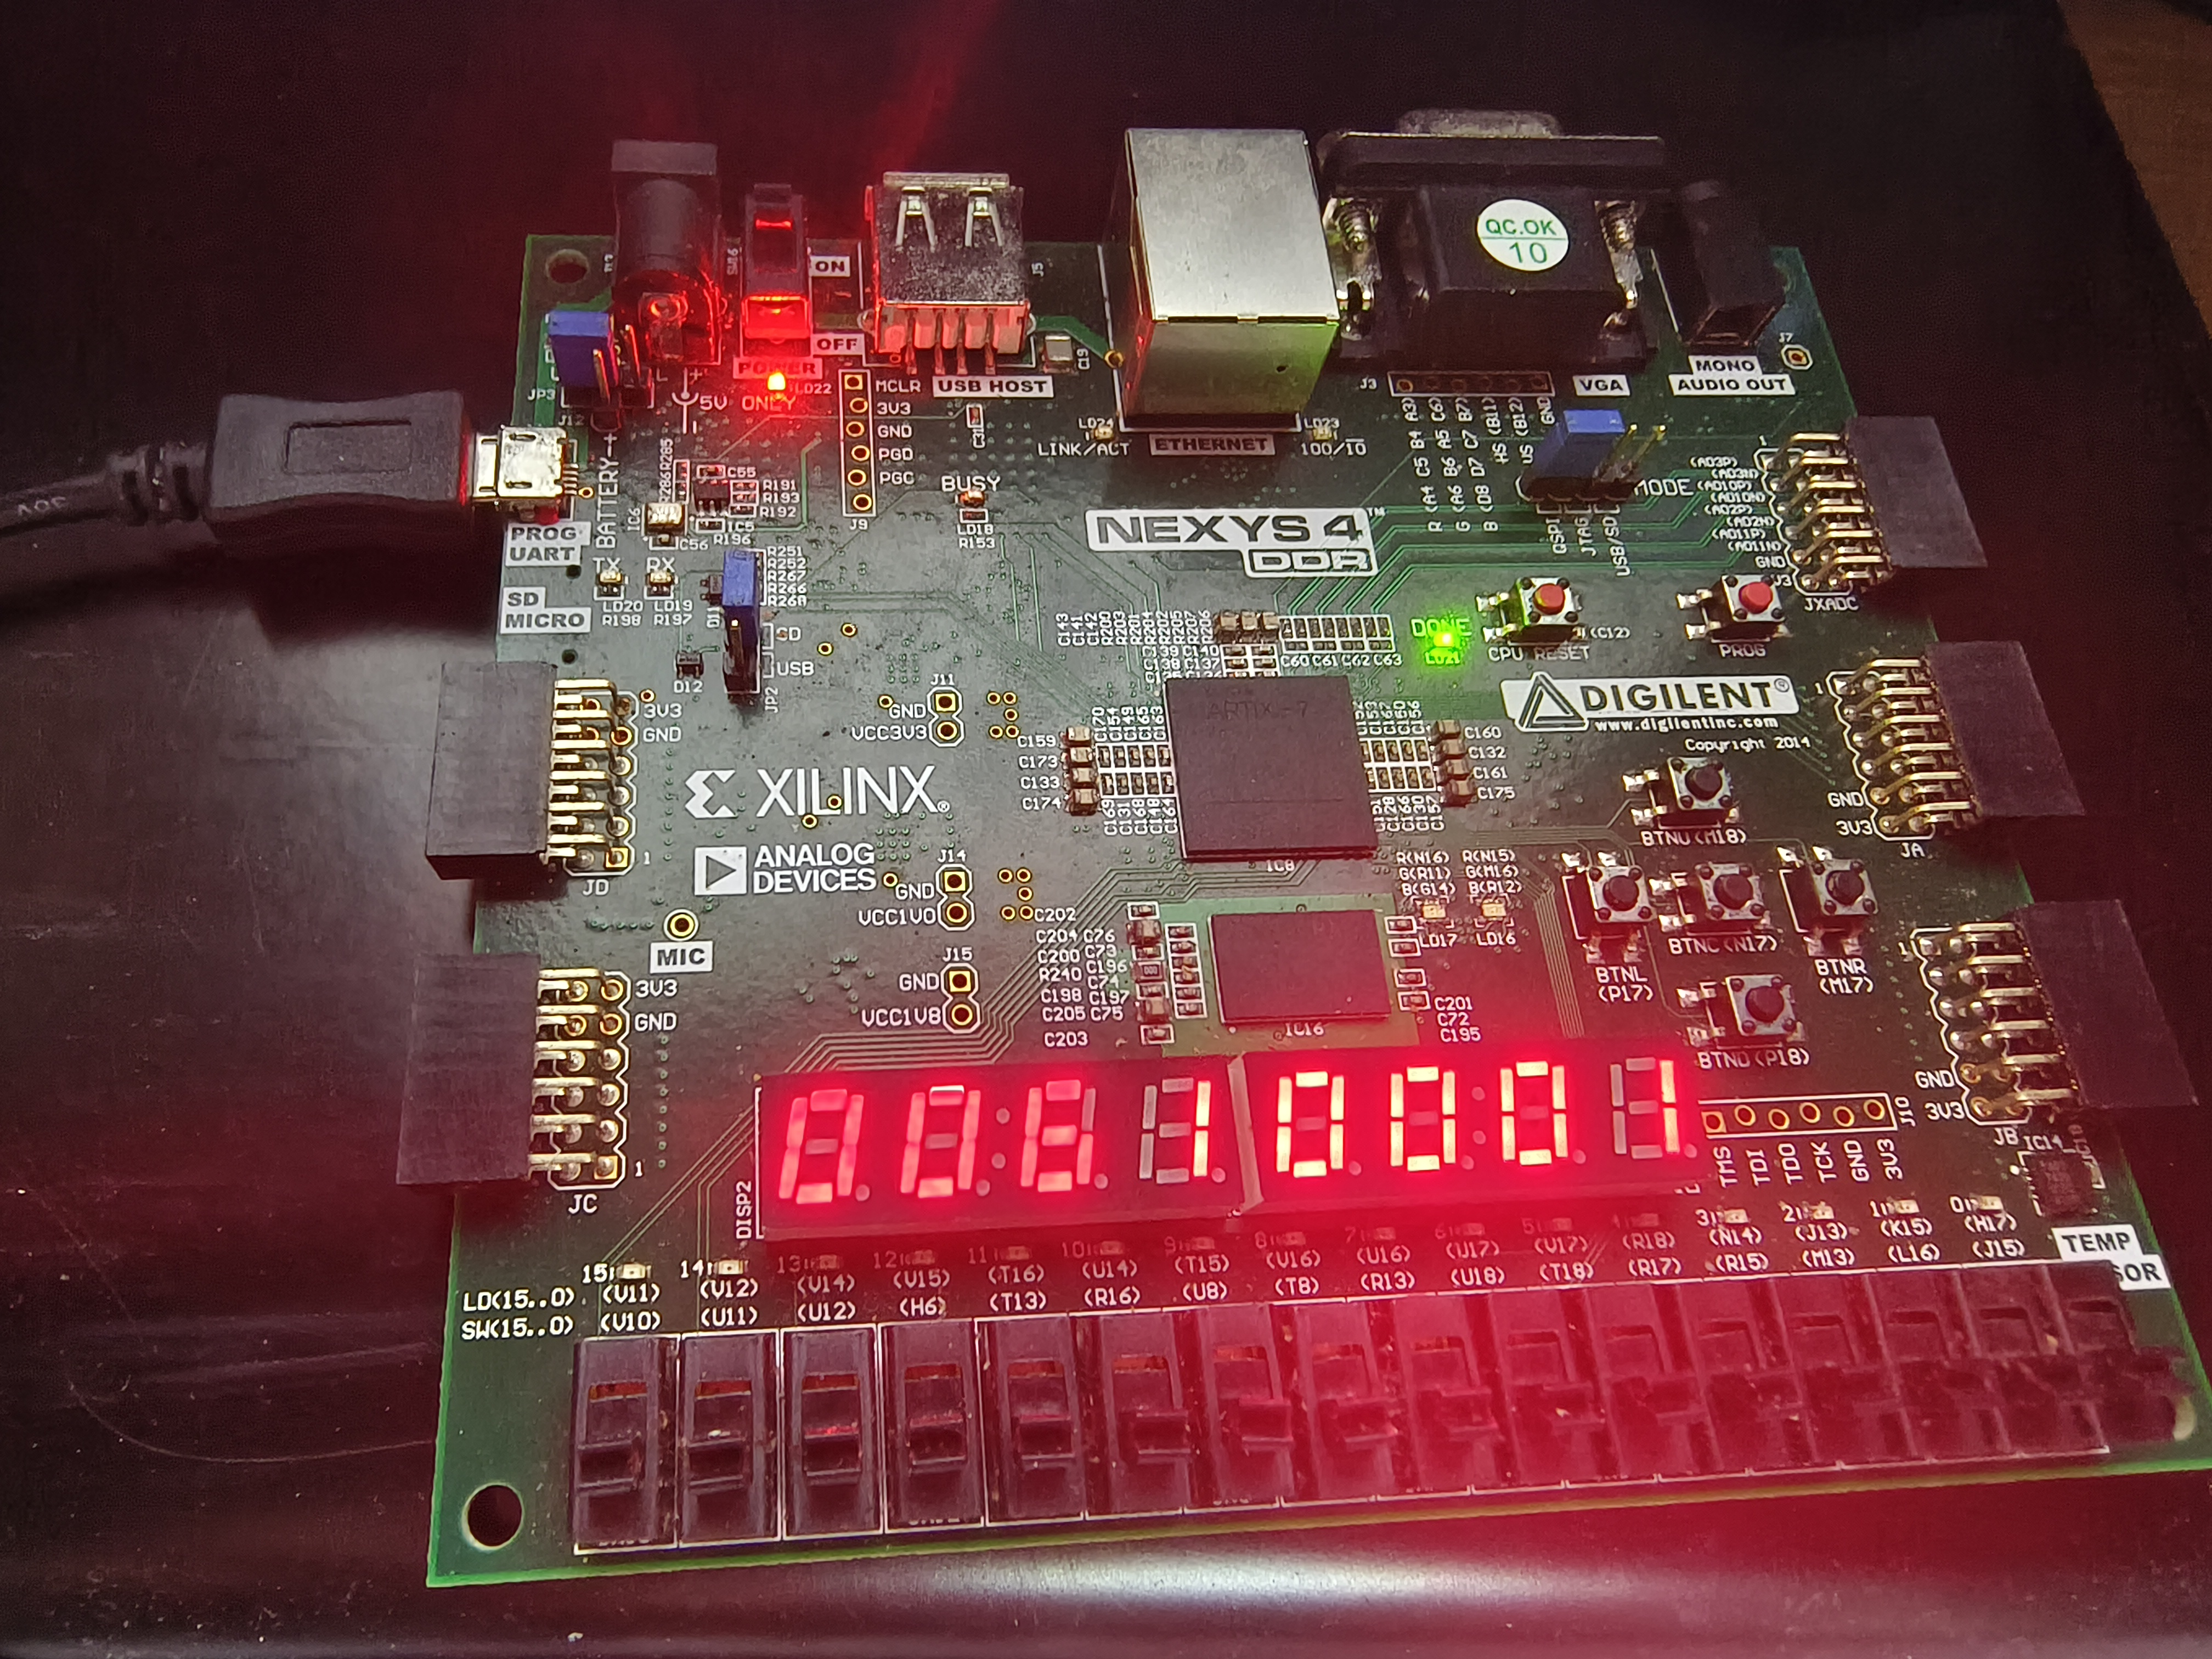
\includegraphics[width=0.6\textwidth]{img/board_result1.jpg}
    \caption{测试通过——数码管低半字显示0001}
\end{figure}

\begin{figure}[H]
    \centering
    % TODO: 替换为数码管高半字递增的开发板实物照片
    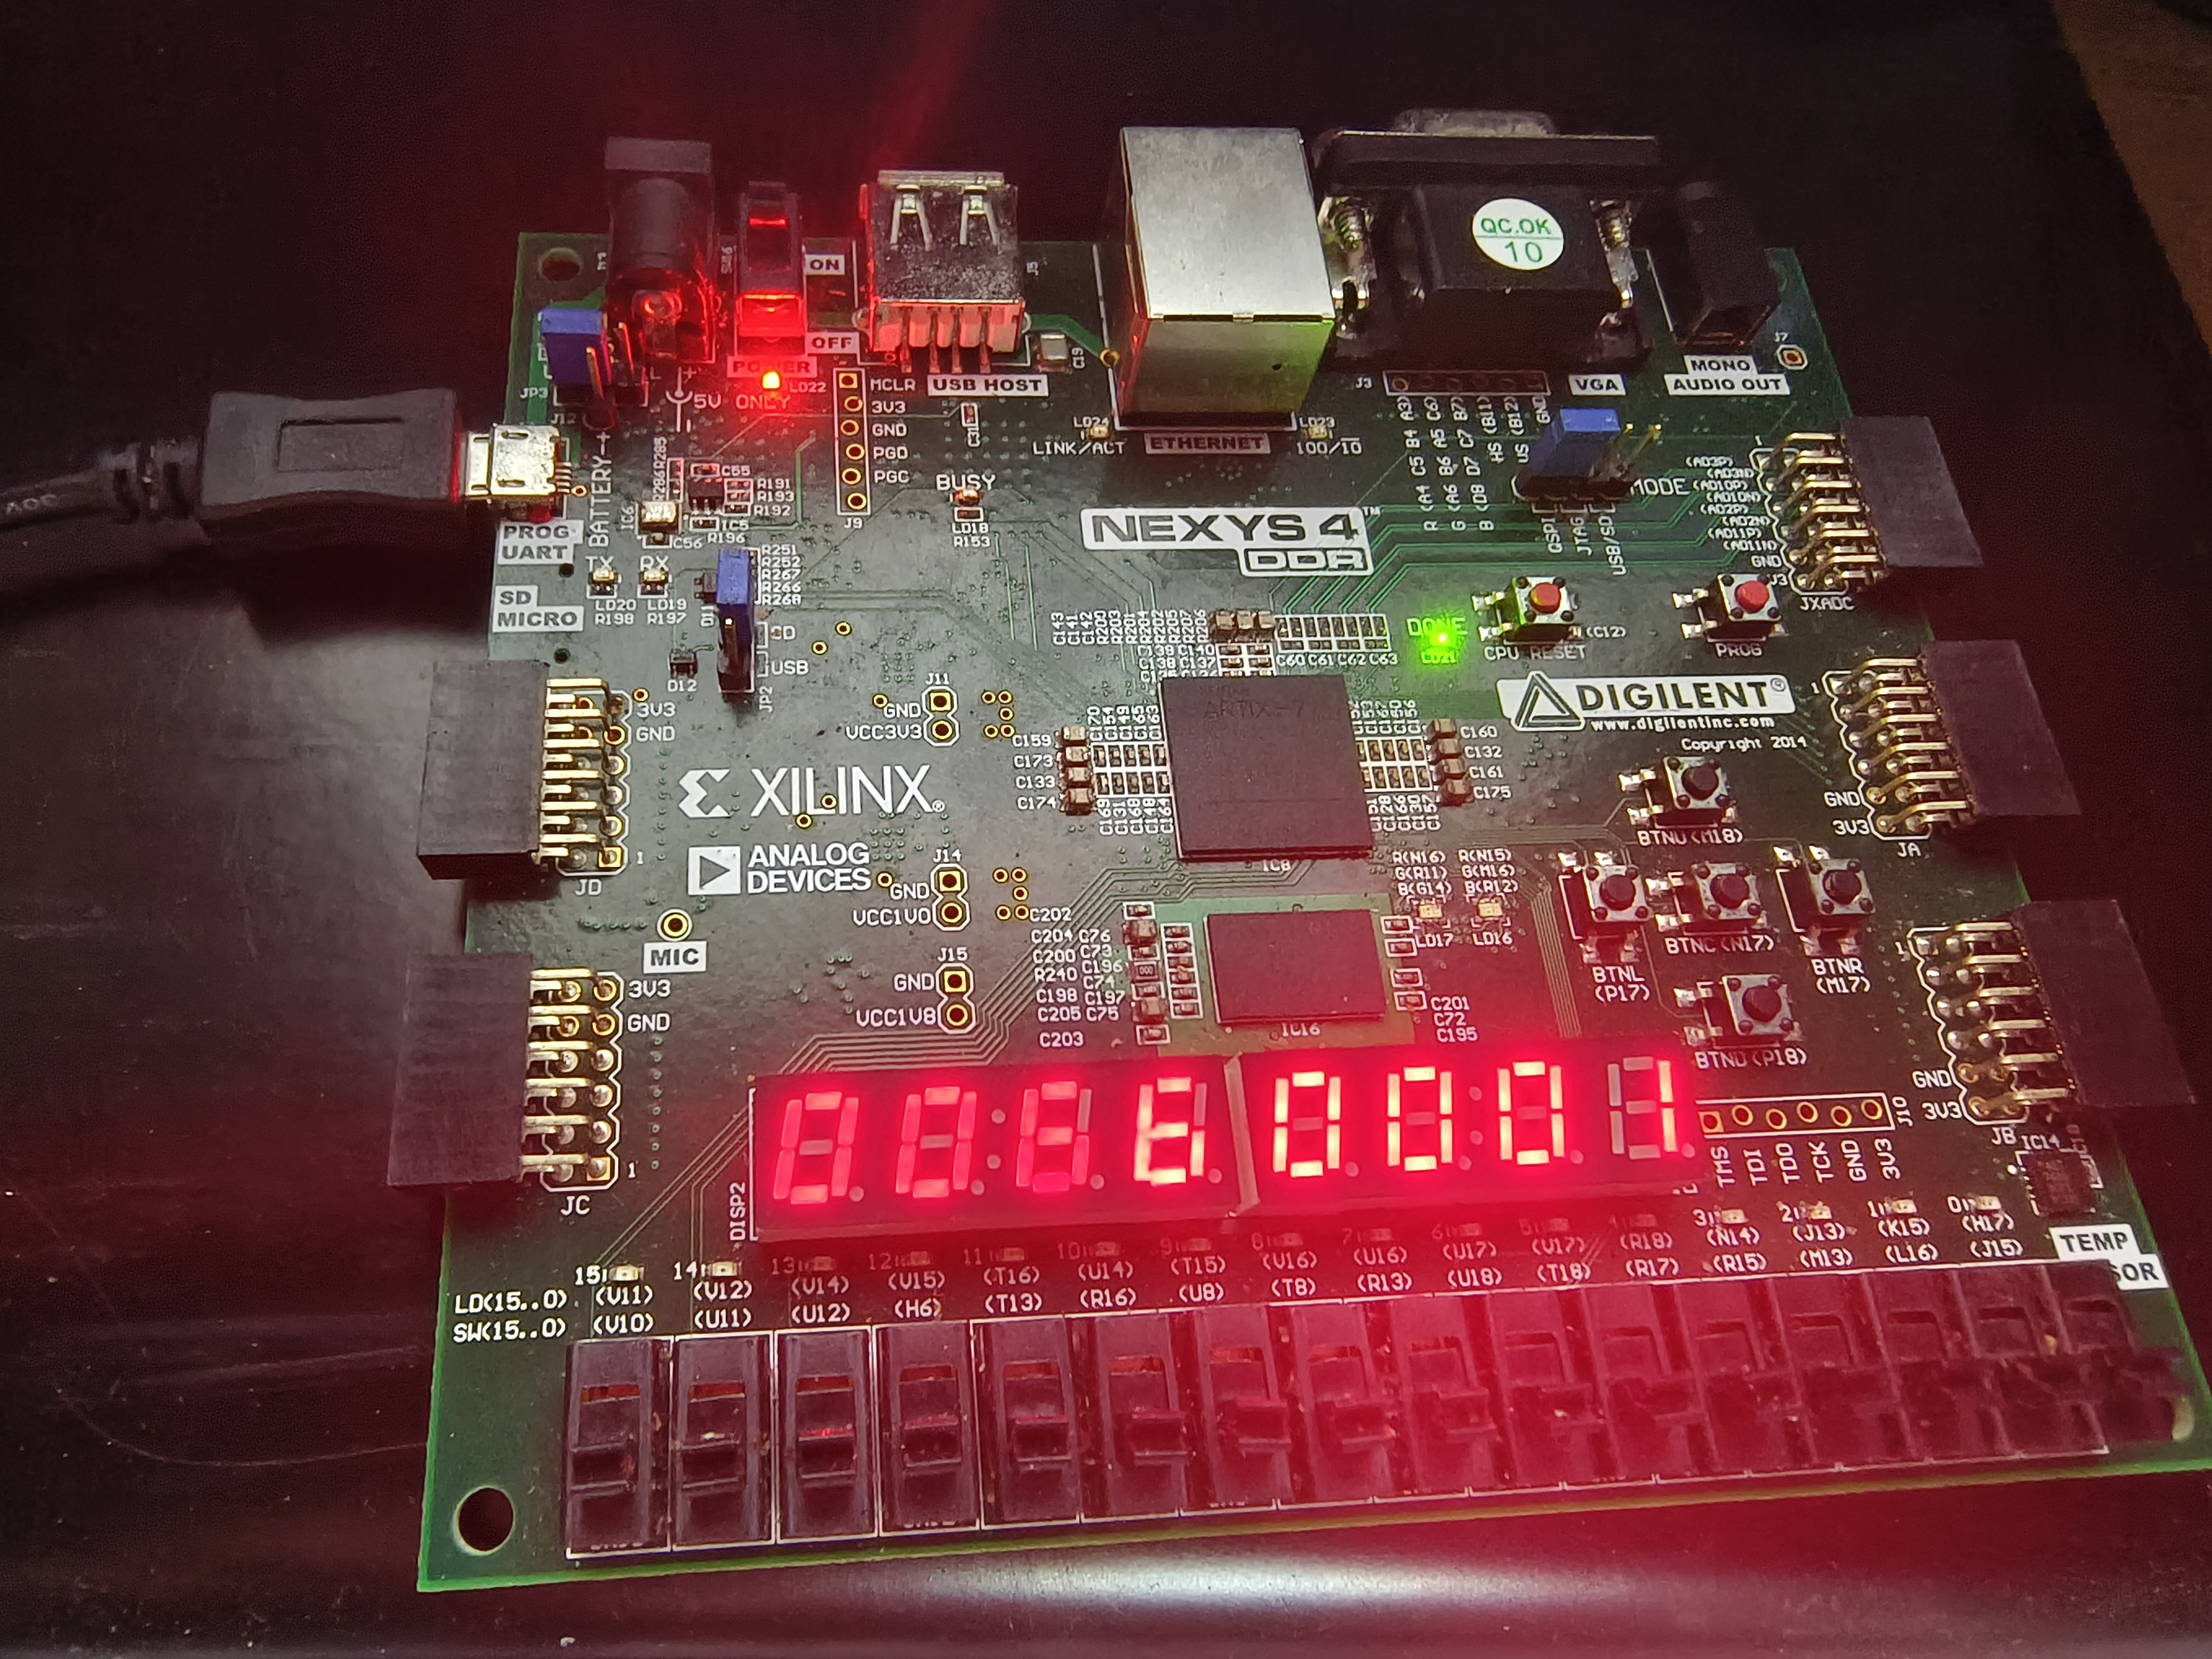
\includegraphics[width=0.6\textwidth]{img/board_result2.jpg}
    \caption{时钟中断正常——数码管高半字持续递增}
\end{figure}
